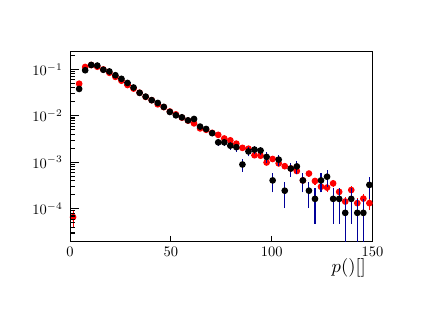
\begin{tikzpicture}
\pgfdeclareplotmark{cross} {
\pgfpathmoveto{\pgfpoint{-0.3\pgfplotmarksize}{\pgfplotmarksize}}
\pgfpathlineto{\pgfpoint{+0.3\pgfplotmarksize}{\pgfplotmarksize}}
\pgfpathlineto{\pgfpoint{+0.3\pgfplotmarksize}{0.3\pgfplotmarksize}}
\pgfpathlineto{\pgfpoint{+1\pgfplotmarksize}{0.3\pgfplotmarksize}}
\pgfpathlineto{\pgfpoint{+1\pgfplotmarksize}{-0.3\pgfplotmarksize}}
\pgfpathlineto{\pgfpoint{+0.3\pgfplotmarksize}{-0.3\pgfplotmarksize}}
\pgfpathlineto{\pgfpoint{+0.3\pgfplotmarksize}{-1.\pgfplotmarksize}}
\pgfpathlineto{\pgfpoint{-0.3\pgfplotmarksize}{-1.\pgfplotmarksize}}
\pgfpathlineto{\pgfpoint{-0.3\pgfplotmarksize}{-0.3\pgfplotmarksize}}
\pgfpathlineto{\pgfpoint{-1.\pgfplotmarksize}{-0.3\pgfplotmarksize}}
\pgfpathlineto{\pgfpoint{-1.\pgfplotmarksize}{0.3\pgfplotmarksize}}
\pgfpathlineto{\pgfpoint{-0.3\pgfplotmarksize}{0.3\pgfplotmarksize}}
\pgfpathclose
\pgfusepathqstroke
}
\pgfdeclareplotmark{cross*} {
\pgfpathmoveto{\pgfpoint{-0.3\pgfplotmarksize}{\pgfplotmarksize}}
\pgfpathlineto{\pgfpoint{+0.3\pgfplotmarksize}{\pgfplotmarksize}}
\pgfpathlineto{\pgfpoint{+0.3\pgfplotmarksize}{0.3\pgfplotmarksize}}
\pgfpathlineto{\pgfpoint{+1\pgfplotmarksize}{0.3\pgfplotmarksize}}
\pgfpathlineto{\pgfpoint{+1\pgfplotmarksize}{-0.3\pgfplotmarksize}}
\pgfpathlineto{\pgfpoint{+0.3\pgfplotmarksize}{-0.3\pgfplotmarksize}}
\pgfpathlineto{\pgfpoint{+0.3\pgfplotmarksize}{-1.\pgfplotmarksize}}
\pgfpathlineto{\pgfpoint{-0.3\pgfplotmarksize}{-1.\pgfplotmarksize}}
\pgfpathlineto{\pgfpoint{-0.3\pgfplotmarksize}{-0.3\pgfplotmarksize}}
\pgfpathlineto{\pgfpoint{-1.\pgfplotmarksize}{-0.3\pgfplotmarksize}}
\pgfpathlineto{\pgfpoint{-1.\pgfplotmarksize}{0.3\pgfplotmarksize}}
\pgfpathlineto{\pgfpoint{-0.3\pgfplotmarksize}{0.3\pgfplotmarksize}}
\pgfpathclose
\pgfusepathqfillstroke
}
\pgfdeclareplotmark{newstar} {
\pgfpathmoveto{\pgfqpoint{0pt}{\pgfplotmarksize}}
\pgfpathlineto{\pgfqpointpolar{44}{0.5\pgfplotmarksize}}
\pgfpathlineto{\pgfqpointpolar{18}{\pgfplotmarksize}}
\pgfpathlineto{\pgfqpointpolar{-20}{0.5\pgfplotmarksize}}
\pgfpathlineto{\pgfqpointpolar{-54}{\pgfplotmarksize}}
\pgfpathlineto{\pgfqpointpolar{-90}{0.5\pgfplotmarksize}}
\pgfpathlineto{\pgfqpointpolar{234}{\pgfplotmarksize}}
\pgfpathlineto{\pgfqpointpolar{198}{0.5\pgfplotmarksize}}
\pgfpathlineto{\pgfqpointpolar{162}{\pgfplotmarksize}}
\pgfpathlineto{\pgfqpointpolar{134}{0.5\pgfplotmarksize}}
\pgfpathclose
\pgfusepathqstroke
}
\pgfdeclareplotmark{newstar*} {
\pgfpathmoveto{\pgfqpoint{0pt}{\pgfplotmarksize}}
\pgfpathlineto{\pgfqpointpolar{44}{0.5\pgfplotmarksize}}
\pgfpathlineto{\pgfqpointpolar{18}{\pgfplotmarksize}}
\pgfpathlineto{\pgfqpointpolar{-20}{0.5\pgfplotmarksize}}
\pgfpathlineto{\pgfqpointpolar{-54}{\pgfplotmarksize}}
\pgfpathlineto{\pgfqpointpolar{-90}{0.5\pgfplotmarksize}}
\pgfpathlineto{\pgfqpointpolar{234}{\pgfplotmarksize}}
\pgfpathlineto{\pgfqpointpolar{198}{0.5\pgfplotmarksize}}
\pgfpathlineto{\pgfqpointpolar{162}{\pgfplotmarksize}}
\pgfpathlineto{\pgfqpointpolar{134}{0.5\pgfplotmarksize}}
\pgfpathclose
\pgfusepathqfillstroke
}
\definecolor{c}{rgb}{1,1,1};
\draw [color=c, fill=c] (5.1,3.20034) rectangle (9.9,6.21242);
\draw [color=c, fill=c] (5.58,3.50154) rectangle (9.42,5.91121);
\definecolor{c}{rgb}{0,0,0};
\draw [c] (5.58,3.50154) -- (5.58,5.91121) -- (9.42,5.91121) -- (9.42,3.50154) -- (5.58,3.50154);
\definecolor{c}{rgb}{1,0,0};
\draw [c] (5.6184,3.67911) -- (5.6184,3.81351);
\draw [c] (5.6184,3.81351) -- (5.6184,3.90121);
\draw [c] (5.58,3.81351) -- (5.6184,3.81351);
\draw [c] (5.6184,3.81351) -- (5.6568,3.81351);
\foreach \P in {(5.6184,3.81351)}{\draw[mark options={color=c,fill=c},mark size=2.402402pt,mark=*,mark size=1pt] plot coordinates {\P};}
\draw [c] (5.6952,5.50389) -- (5.6952,5.50775);
\draw [c] (5.6952,5.50775) -- (5.6952,5.51156);
\draw [c] (5.6568,5.50775) -- (5.6952,5.50775);
\draw [c] (5.6952,5.50775) -- (5.7336,5.50775);
\foreach \P in {(5.6952,5.50775)}{\draw[mark options={color=c,fill=c},mark size=2.402402pt,mark=*,mark size=1pt] plot coordinates {\P};}
\draw [c] (5.772,5.71769) -- (5.772,5.72023);
\draw [c] (5.772,5.72023) -- (5.772,5.72275);
\draw [c] (5.7336,5.72023) -- (5.772,5.72023);
\draw [c] (5.772,5.72023) -- (5.8104,5.72023);
\foreach \P in {(5.772,5.72023)}{\draw[mark options={color=c,fill=c},mark size=2.402402pt,mark=*,mark size=1pt] plot coordinates {\P};}
\draw [c] (5.8488,5.74268) -- (5.8488,5.7451);
\draw [c] (5.8488,5.7451) -- (5.8488,5.7475);
\draw [c] (5.8104,5.7451) -- (5.8488,5.7451);
\draw [c] (5.8488,5.7451) -- (5.8872,5.7451);
\foreach \P in {(5.8488,5.7451)}{\draw[mark options={color=c,fill=c},mark size=2.402402pt,mark=*,mark size=1pt] plot coordinates {\P};}
\draw [c] (5.9256,5.72103) -- (5.9256,5.72356);
\draw [c] (5.9256,5.72356) -- (5.9256,5.72606);
\draw [c] (5.8872,5.72356) -- (5.9256,5.72356);
\draw [c] (5.9256,5.72356) -- (5.964,5.72356);
\foreach \P in {(5.9256,5.72356)}{\draw[mark options={color=c,fill=c},mark size=2.402402pt,mark=*,mark size=1pt] plot coordinates {\P};}
\draw [c] (6.0024,5.68602) -- (6.0024,5.68873);
\draw [c] (6.0024,5.68873) -- (6.0024,5.69141);
\draw [c] (5.964,5.68873) -- (6.0024,5.68873);
\draw [c] (6.0024,5.68873) -- (6.0408,5.68873);
\foreach \P in {(6.0024,5.68873)}{\draw[mark options={color=c,fill=c},mark size=2.402402pt,mark=*,mark size=1pt] plot coordinates {\P};}
\draw [c] (6.0792,5.64398) -- (6.0792,5.64692);
\draw [c] (6.0792,5.64692) -- (6.0792,5.64982);
\draw [c] (6.0408,5.64692) -- (6.0792,5.64692);
\draw [c] (6.0792,5.64692) -- (6.1176,5.64692);
\foreach \P in {(6.0792,5.64692)}{\draw[mark options={color=c,fill=c},mark size=2.402402pt,mark=*,mark size=1pt] plot coordinates {\P};}
\draw [c] (6.156,5.59152) -- (6.156,5.59477);
\draw [c] (6.156,5.59477) -- (6.156,5.59798);
\draw [c] (6.1176,5.59477) -- (6.156,5.59477);
\draw [c] (6.156,5.59477) -- (6.1944,5.59477);
\foreach \P in {(6.156,5.59477)}{\draw[mark options={color=c,fill=c},mark size=2.402402pt,mark=*,mark size=1pt] plot coordinates {\P};}
\draw [c] (6.2328,5.54246) -- (6.2328,5.54604);
\draw [c] (6.2328,5.54604) -- (6.2328,5.54957);
\draw [c] (6.1944,5.54604) -- (6.2328,5.54604);
\draw [c] (6.2328,5.54604) -- (6.2712,5.54604);
\foreach \P in {(6.2328,5.54604)}{\draw[mark options={color=c,fill=c},mark size=2.402402pt,mark=*,mark size=1pt] plot coordinates {\P};}
\draw [c] (6.3096,5.48726) -- (6.3096,5.49125);
\draw [c] (6.3096,5.49125) -- (6.3096,5.49518);
\draw [c] (6.2712,5.49125) -- (6.3096,5.49125);
\draw [c] (6.3096,5.49125) -- (6.348,5.49125);
\foreach \P in {(6.3096,5.49125)}{\draw[mark options={color=c,fill=c},mark size=2.402402pt,mark=*,mark size=1pt] plot coordinates {\P};}
\draw [c] (6.3864,5.44142) -- (6.3864,5.44578);
\draw [c] (6.3864,5.44578) -- (6.3864,5.45006);
\draw [c] (6.348,5.44578) -- (6.3864,5.44578);
\draw [c] (6.3864,5.44578) -- (6.4248,5.44578);
\foreach \P in {(6.3864,5.44578)}{\draw[mark options={color=c,fill=c},mark size=2.402402pt,mark=*,mark size=1pt] plot coordinates {\P};}
\draw [c] (6.4632,5.38859) -- (6.4632,5.39342);
\draw [c] (6.4632,5.39342) -- (6.4632,5.39817);
\draw [c] (6.4248,5.39342) -- (6.4632,5.39342);
\draw [c] (6.4632,5.39342) -- (6.5016,5.39342);
\foreach \P in {(6.4632,5.39342)}{\draw[mark options={color=c,fill=c},mark size=2.402402pt,mark=*,mark size=1pt] plot coordinates {\P};}
\draw [c] (6.54,5.33504) -- (6.54,5.34041);
\draw [c] (6.54,5.34041) -- (6.54,5.34567);
\draw [c] (6.5016,5.34041) -- (6.54,5.34041);
\draw [c] (6.54,5.34041) -- (6.5784,5.34041);
\foreach \P in {(6.54,5.34041)}{\draw[mark options={color=c,fill=c},mark size=2.402402pt,mark=*,mark size=1pt] plot coordinates {\P};}
\draw [c] (6.6168,5.29257) -- (6.6168,5.2984);
\draw [c] (6.6168,5.2984) -- (6.6168,5.3041);
\draw [c] (6.5784,5.2984) -- (6.6168,5.2984);
\draw [c] (6.6168,5.2984) -- (6.6552,5.2984);
\foreach \P in {(6.6168,5.2984)}{\draw[mark options={color=c,fill=c},mark size=2.402402pt,mark=*,mark size=1pt] plot coordinates {\P};}
\draw [c] (6.6936,5.23943) -- (6.6936,5.24589);
\draw [c] (6.6936,5.24589) -- (6.6936,5.2522);
\draw [c] (6.6552,5.24589) -- (6.6936,5.24589);
\draw [c] (6.6936,5.24589) -- (6.732,5.24589);
\foreach \P in {(6.6936,5.24589)}{\draw[mark options={color=c,fill=c},mark size=2.402402pt,mark=*,mark size=1pt] plot coordinates {\P};}
\draw [c] (6.7704,5.20368) -- (6.7704,5.21062);
\draw [c] (6.7704,5.21062) -- (6.7704,5.21737);
\draw [c] (6.732,5.21062) -- (6.7704,5.21062);
\draw [c] (6.7704,5.21062) -- (6.8088,5.21062);
\foreach \P in {(6.7704,5.21062)}{\draw[mark options={color=c,fill=c},mark size=2.402402pt,mark=*,mark size=1pt] plot coordinates {\P};}
\draw [c] (6.8472,5.14694) -- (6.8472,5.15468);
\draw [c] (6.8472,5.15468) -- (6.8472,5.1622);
\draw [c] (6.8088,5.15468) -- (6.8472,5.15468);
\draw [c] (6.8472,5.15468) -- (6.8856,5.15468);
\foreach \P in {(6.8472,5.15468)}{\draw[mark options={color=c,fill=c},mark size=2.402402pt,mark=*,mark size=1pt] plot coordinates {\P};}
\draw [c] (6.924,5.10977) -- (6.924,5.1181);
\draw [c] (6.924,5.1181) -- (6.924,5.12616);
\draw [c] (6.8856,5.1181) -- (6.924,5.1181);
\draw [c] (6.924,5.1181) -- (6.9624,5.1181);
\foreach \P in {(6.924,5.1181)}{\draw[mark options={color=c,fill=c},mark size=2.402402pt,mark=*,mark size=1pt] plot coordinates {\P};}
\draw [c] (7.0008,5.06759) -- (7.0008,5.07663);
\draw [c] (7.0008,5.07663) -- (7.0008,5.08537);
\draw [c] (6.9624,5.07663) -- (7.0008,5.07663);
\draw [c] (7.0008,5.07663) -- (7.0392,5.07663);
\foreach \P in {(7.0008,5.07663)}{\draw[mark options={color=c,fill=c},mark size=2.402402pt,mark=*,mark size=1pt] plot coordinates {\P};}
\draw [c] (7.0776,5.02909) -- (7.0776,5.03884);
\draw [c] (7.0776,5.03884) -- (7.0776,5.04823);
\draw [c] (7.0392,5.03884) -- (7.0776,5.03884);
\draw [c] (7.0776,5.03884) -- (7.116,5.03884);
\foreach \P in {(7.0776,5.03884)}{\draw[mark options={color=c,fill=c},mark size=2.402402pt,mark=*,mark size=1pt] plot coordinates {\P};}
\draw [c] (7.1544,4.99362) -- (7.1544,5.00407);
\draw [c] (7.1544,5.00407) -- (7.1544,5.01411);
\draw [c] (7.116,5.00407) -- (7.1544,5.00407);
\draw [c] (7.1544,5.00407) -- (7.1928,5.00407);
\foreach \P in {(7.1544,5.00407)}{\draw[mark options={color=c,fill=c},mark size=2.402402pt,mark=*,mark size=1pt] plot coordinates {\P};}
\draw [c] (7.2312,4.92841) -- (7.2312,4.94027);
\draw [c] (7.2312,4.94027) -- (7.2312,4.95161);
\draw [c] (7.1928,4.94027) -- (7.2312,4.94027);
\draw [c] (7.2312,4.94027) -- (7.2696,4.94027);
\foreach \P in {(7.2312,4.94027)}{\draw[mark options={color=c,fill=c},mark size=2.402402pt,mark=*,mark size=1pt] plot coordinates {\P};}
\draw [c] (7.308,4.91004) -- (7.308,4.92234);
\draw [c] (7.308,4.92234) -- (7.308,4.93407);
\draw [c] (7.2696,4.92234) -- (7.308,4.92234);
\draw [c] (7.308,4.92234) -- (7.3464,4.92234);
\foreach \P in {(7.308,4.92234)}{\draw[mark options={color=c,fill=c},mark size=2.402402pt,mark=*,mark size=1pt] plot coordinates {\P};}
\draw [c] (7.3848,4.87021) -- (7.3848,4.8835);
\draw [c] (7.3848,4.8835) -- (7.3848,4.89614);
\draw [c] (7.3464,4.8835) -- (7.3848,4.8835);
\draw [c] (7.3848,4.8835) -- (7.4232,4.8835);
\foreach \P in {(7.3848,4.8835)}{\draw[mark options={color=c,fill=c},mark size=2.402402pt,mark=*,mark size=1pt] plot coordinates {\P};}
\draw [c] (7.4616,4.84405) -- (7.4616,4.85804);
\draw [c] (7.4616,4.85804) -- (7.4616,4.8713);
\draw [c] (7.4232,4.85804) -- (7.4616,4.85804);
\draw [c] (7.4616,4.85804) -- (7.5,4.85804);
\foreach \P in {(7.4616,4.85804)}{\draw[mark options={color=c,fill=c},mark size=2.402402pt,mark=*,mark size=1pt] plot coordinates {\P};}
\draw [c] (7.5384,4.79686) -- (7.5384,4.8122);
\draw [c] (7.5384,4.8122) -- (7.5384,4.82667);
\draw [c] (7.5,4.8122) -- (7.5384,4.8122);
\draw [c] (7.5384,4.8122) -- (7.5768,4.8122);
\foreach \P in {(7.5384,4.8122)}{\draw[mark options={color=c,fill=c},mark size=2.402402pt,mark=*,mark size=1pt] plot coordinates {\P};}
\draw [c] (7.6152,4.77256) -- (7.6152,4.78865);
\draw [c] (7.6152,4.78865) -- (7.6152,4.80378);
\draw [c] (7.5768,4.78865) -- (7.6152,4.78865);
\draw [c] (7.6152,4.78865) -- (7.6536,4.78865);
\foreach \P in {(7.6152,4.78865)}{\draw[mark options={color=c,fill=c},mark size=2.402402pt,mark=*,mark size=1pt] plot coordinates {\P};}
\draw [c] (7.692,4.72895) -- (7.692,4.74646);
\draw [c] (7.692,4.74646) -- (7.692,4.76285);
\draw [c] (7.6536,4.74646) -- (7.692,4.74646);
\draw [c] (7.692,4.74646) -- (7.7304,4.74646);
\foreach \P in {(7.692,4.74646)}{\draw[mark options={color=c,fill=c},mark size=2.402402pt,mark=*,mark size=1pt] plot coordinates {\P};}
\draw [c] (7.7688,4.67367) -- (7.7688,4.69318);
\draw [c] (7.7688,4.69318) -- (7.7688,4.71131);
\draw [c] (7.7304,4.69318) -- (7.7688,4.69318);
\draw [c] (7.7688,4.69318) -- (7.8072,4.69318);
\foreach \P in {(7.7688,4.69318)}{\draw[mark options={color=c,fill=c},mark size=2.402402pt,mark=*,mark size=1pt] plot coordinates {\P};}
\draw [c] (7.8456,4.66196) -- (7.8456,4.68192);
\draw [c] (7.8456,4.68192) -- (7.8456,4.70044);
\draw [c] (7.8072,4.68192) -- (7.8456,4.68192);
\draw [c] (7.8456,4.68192) -- (7.884,4.68192);
\foreach \P in {(7.8456,4.68192)}{\draw[mark options={color=c,fill=c},mark size=2.402402pt,mark=*,mark size=1pt] plot coordinates {\P};}
\draw [c] (7.9224,4.57583) -- (7.9224,4.59944);
\draw [c] (7.9224,4.59944) -- (7.9224,4.62106);
\draw [c] (7.884,4.59944) -- (7.9224,4.59944);
\draw [c] (7.9224,4.59944) -- (7.9608,4.59944);
\foreach \P in {(7.9224,4.59944)}{\draw[mark options={color=c,fill=c},mark size=2.402402pt,mark=*,mark size=1pt] plot coordinates {\P};}
\draw [c] (7.9992,4.56951) -- (7.9992,4.59341);
\draw [c] (7.9992,4.59341) -- (7.9992,4.61527);
\draw [c] (7.9608,4.59341) -- (7.9992,4.59341);
\draw [c] (7.9992,4.59341) -- (8.0376,4.59341);
\foreach \P in {(7.9992,4.59341)}{\draw[mark options={color=c,fill=c},mark size=2.402402pt,mark=*,mark size=1pt] plot coordinates {\P};}
\draw [c] (8.076,4.47869) -- (8.076,4.50722);
\draw [c] (8.076,4.50722) -- (8.076,4.53289);
\draw [c] (8.0376,4.50722) -- (8.076,4.50722);
\draw [c] (8.076,4.50722) -- (8.1144,4.50722);
\foreach \P in {(8.076,4.50722)}{\draw[mark options={color=c,fill=c},mark size=2.402402pt,mark=*,mark size=1pt] plot coordinates {\P};}
\draw [c] (8.1528,4.5255) -- (8.1528,4.55154);
\draw [c] (8.1528,4.55154) -- (8.1528,4.57518);
\draw [c] (8.1144,4.55154) -- (8.1528,4.55154);
\draw [c] (8.1528,4.55154) -- (8.1912,4.55154);
\foreach \P in {(8.1528,4.55154)}{\draw[mark options={color=c,fill=c},mark size=2.402402pt,mark=*,mark size=1pt] plot coordinates {\P};}
\draw [c] (8.2296,4.46635) -- (8.2296,4.49557);
\draw [c] (8.2296,4.49557) -- (8.2296,4.52181);
\draw [c] (8.1912,4.49557) -- (8.2296,4.49557);
\draw [c] (8.2296,4.49557) -- (8.268,4.49557);
\foreach \P in {(8.2296,4.49557)}{\draw[mark options={color=c,fill=c},mark size=2.402402pt,mark=*,mark size=1pt] plot coordinates {\P};}
\draw [c] (8.3064,4.42908) -- (8.3064,4.46052);
\draw [c] (8.3064,4.46052) -- (8.3064,4.48851);
\draw [c] (8.268,4.46052) -- (8.3064,4.46052);
\draw [c] (8.3064,4.46052) -- (8.3448,4.46052);
\foreach \P in {(8.3064,4.46052)}{\draw[mark options={color=c,fill=c},mark size=2.402402pt,mark=*,mark size=1pt] plot coordinates {\P};}
\draw [c] (8.3832,4.39824) -- (8.3832,4.43162);
\draw [c] (8.3832,4.43162) -- (8.3832,4.46115);
\draw [c] (8.3448,4.43162) -- (8.3832,4.43162);
\draw [c] (8.3832,4.43162) -- (8.4216,4.43162);
\foreach \P in {(8.3832,4.43162)}{\draw[mark options={color=c,fill=c},mark size=2.402402pt,mark=*,mark size=1pt] plot coordinates {\P};}
\draw [c] (8.46,4.36332) -- (8.46,4.39905);
\draw [c] (8.46,4.39905) -- (8.46,4.4304);
\draw [c] (8.4216,4.39905) -- (8.46,4.39905);
\draw [c] (8.46,4.39905) -- (8.4984,4.39905);
\foreach \P in {(8.46,4.39905)}{\draw[mark options={color=c,fill=c},mark size=2.402402pt,mark=*,mark size=1pt] plot coordinates {\P};}
\draw [c] (8.5368,4.23351) -- (8.5368,4.27952);
\draw [c] (8.5368,4.27952) -- (8.5368,4.31851);
\draw [c] (8.4984,4.27952) -- (8.5368,4.27952);
\draw [c] (8.5368,4.27952) -- (8.5752,4.27952);
\foreach \P in {(8.5368,4.27952)}{\draw[mark options={color=c,fill=c},mark size=2.402402pt,mark=*,mark size=1pt] plot coordinates {\P};}
\draw [c] (8.6136,4.32845) -- (8.6136,4.3667);
\draw [c] (8.6136,4.3667) -- (8.6136,4.39996);
\draw [c] (8.5752,4.3667) -- (8.6136,4.3667);
\draw [c] (8.6136,4.3667) -- (8.652,4.3667);
\foreach \P in {(8.6136,4.3667)}{\draw[mark options={color=c,fill=c},mark size=2.402402pt,mark=*,mark size=1pt] plot coordinates {\P};}
\draw [c] (8.6904,4.22579) -- (8.6904,4.2725);
\draw [c] (8.6904,4.2725) -- (8.6904,4.31199);
\draw [c] (8.652,4.2725) -- (8.6904,4.2725);
\draw [c] (8.6904,4.2725) -- (8.7288,4.2725);
\foreach \P in {(8.6904,4.2725)}{\draw[mark options={color=c,fill=c},mark size=2.402402pt,mark=*,mark size=1pt] plot coordinates {\P};}
\draw [c] (8.7672,4.14405) -- (8.7672,4.1988);
\draw [c] (8.7672,4.1988) -- (8.7672,4.24389);
\draw [c] (8.7288,4.1988) -- (8.7672,4.1988);
\draw [c] (8.7672,4.1988) -- (8.8056,4.1988);
\foreach \P in {(8.7672,4.1988)}{\draw[mark options={color=c,fill=c},mark size=2.402402pt,mark=*,mark size=1pt] plot coordinates {\P};}
\draw [c] (8.844,4.13321) -- (8.844,4.18914);
\draw [c] (8.844,4.18914) -- (8.844,4.23501);
\draw [c] (8.8056,4.18914) -- (8.844,4.18914);
\draw [c] (8.844,4.18914) -- (8.8824,4.18914);
\foreach \P in {(8.844,4.18914)}{\draw[mark options={color=c,fill=c},mark size=2.402402pt,mark=*,mark size=1pt] plot coordinates {\P};}
\draw [c] (8.9208,4.19249) -- (8.9208,4.24233);
\draw [c] (8.9208,4.24233) -- (8.9208,4.28402);
\draw [c] (8.8824,4.24233) -- (8.9208,4.24233);
\draw [c] (8.9208,4.24233) -- (8.9592,4.24233);
\foreach \P in {(8.9208,4.24233)}{\draw[mark options={color=c,fill=c},mark size=2.402402pt,mark=*,mark size=1pt] plot coordinates {\P};}
\draw [c] (8.9976,4.07136) -- (8.9976,4.13442);
\draw [c] (8.9976,4.13442) -- (8.9976,4.18499);
\draw [c] (8.9592,4.13442) -- (8.9976,4.13442);
\draw [c] (8.9976,4.13442) -- (9.036,4.13442);
\foreach \P in {(8.9976,4.13442)}{\draw[mark options={color=c,fill=c},mark size=2.402402pt,mark=*,mark size=1pt] plot coordinates {\P};}
\draw [c] (9.0744,3.92836) -- (9.0744,4.01157);
\draw [c] (9.0744,4.01157) -- (9.0744,4.07428);
\draw [c] (9.036,4.01157) -- (9.0744,4.01157);
\draw [c] (9.0744,4.01157) -- (9.1128,4.01157);
\foreach \P in {(9.0744,4.01157)}{\draw[mark options={color=c,fill=c},mark size=2.402402pt,mark=*,mark size=1pt] plot coordinates {\P};}
\draw [c] (9.1512,4.09783) -- (9.1512,4.15773);
\draw [c] (9.1512,4.15773) -- (9.1512,4.20624);
\draw [c] (9.1128,4.15773) -- (9.1512,4.15773);
\draw [c] (9.1512,4.15773) -- (9.1896,4.15773);
\foreach \P in {(9.1512,4.15773)}{\draw[mark options={color=c,fill=c},mark size=2.402402pt,mark=*,mark size=1pt] plot coordinates {\P};}
\draw [c] (9.228,3.90381) -- (9.228,3.99107);
\draw [c] (9.228,3.99107) -- (9.228,4.05604);
\draw [c] (9.1896,3.99107) -- (9.228,3.99107);
\draw [c] (9.228,3.99107) -- (9.2664,3.99107);
\foreach \P in {(9.228,3.99107)}{\draw[mark options={color=c,fill=c},mark size=2.402402pt,mark=*,mark size=1pt] plot coordinates {\P};}
\draw [c] (9.3048,3.97172) -- (9.3048,4.04823);
\draw [c] (9.3048,4.04823) -- (9.3048,4.10707);
\draw [c] (9.2664,4.04823) -- (9.3048,4.04823);
\draw [c] (9.3048,4.04823) -- (9.3432,4.04823);
\foreach \P in {(9.3048,4.04823)}{\draw[mark options={color=c,fill=c},mark size=2.402402pt,mark=*,mark size=1pt] plot coordinates {\P};}
\draw [c] (9.3816,3.90381) -- (9.3816,3.99107);
\draw [c] (9.3816,3.99107) -- (9.3816,4.05604);
\draw [c] (9.3432,3.99107) -- (9.3816,3.99107);
\draw [c] (9.3816,3.99107) -- (9.42,3.99107);
\foreach \P in {(9.3816,3.99107)}{\draw[mark options={color=c,fill=c},mark size=2.402402pt,mark=*,mark size=1pt] plot coordinates {\P};}
\definecolor{c}{rgb}{0,0,0};
\draw [c] (5.58,3.50154) -- (9.42,3.50154);
\draw [anchor= east] (9.42,3.16419) node[scale=0.672711, rotate=0]{$p(\pion) [\mevc]$};
\draw [c] (5.58,3.57383) -- (5.58,3.50154);
\draw [c] (6.86,3.57383) -- (6.86,3.50154);
\draw [c] (8.14,3.57383) -- (8.14,3.50154);
\draw [c] (9.42,3.57383) -- (9.42,3.50154);
\draw [anchor=base] (5.58,3.30877) node[scale=0.52322, rotate=0]{0};
\draw [anchor=base] (6.86,3.30877) node[scale=0.52322, rotate=0]{50};
\draw [anchor=base] (8.14,3.30877) node[scale=0.52322, rotate=0]{100};
\draw [anchor=base] (9.42,3.30877) node[scale=0.52322, rotate=0]{150};
\draw [c] (5.58,3.50154) -- (5.58,5.91121);
\draw [c] (5.6376,3.50734) -- (5.58,3.50734);
\draw [c] (5.6376,3.61121) -- (5.58,3.61121);
\draw [c] (5.6376,3.6849) -- (5.58,3.6849);
\draw [c] (5.6376,3.74207) -- (5.58,3.74207);
\draw [c] (5.6376,3.78877) -- (5.58,3.78877);
\draw [c] (5.6376,3.82826) -- (5.58,3.82826);
\draw [c] (5.6376,3.86247) -- (5.58,3.86247);
\draw [c] (5.6376,3.89264) -- (5.58,3.89264);
\draw [c] (5.6952,3.91963) -- (5.58,3.91963);
\draw [anchor= east] (5.54928,3.91963) node[scale=0.52322, rotate=0]{$10^{-4}$};
\draw [c] (5.6376,4.09719) -- (5.58,4.09719);
\draw [c] (5.6376,4.20106) -- (5.58,4.20106);
\draw [c] (5.6376,4.27475) -- (5.58,4.27475);
\draw [c] (5.6376,4.33191) -- (5.58,4.33191);
\draw [c] (5.6376,4.37862) -- (5.58,4.37862);
\draw [c] (5.6376,4.41811) -- (5.58,4.41811);
\draw [c] (5.6376,4.45231) -- (5.58,4.45231);
\draw [c] (5.6376,4.48248) -- (5.58,4.48248);
\draw [c] (5.6952,4.50947) -- (5.58,4.50947);
\draw [anchor= east] (5.54928,4.50947) node[scale=0.52322, rotate=0]{$10^{-3}$};
\draw [c] (5.6376,4.68704) -- (5.58,4.68704);
\draw [c] (5.6376,4.7909) -- (5.58,4.7909);
\draw [c] (5.6376,4.8646) -- (5.58,4.8646);
\draw [c] (5.6376,4.92176) -- (5.58,4.92176);
\draw [c] (5.6376,4.96846) -- (5.58,4.96846);
\draw [c] (5.6376,5.00795) -- (5.58,5.00795);
\draw [c] (5.6376,5.04216) -- (5.58,5.04216);
\draw [c] (5.6376,5.07233) -- (5.58,5.07233);
\draw [c] (5.6952,5.09932) -- (5.58,5.09932);
\draw [anchor= east] (5.54928,5.09932) node[scale=0.52322, rotate=0]{$10^{-2}$};
\draw [c] (5.6376,5.27688) -- (5.58,5.27688);
\draw [c] (5.6376,5.38075) -- (5.58,5.38075);
\draw [c] (5.6376,5.45444) -- (5.58,5.45444);
\draw [c] (5.6376,5.5116) -- (5.58,5.5116);
\draw [c] (5.6376,5.55831) -- (5.58,5.55831);
\draw [c] (5.6376,5.5978) -- (5.58,5.5978);
\draw [c] (5.6376,5.632) -- (5.58,5.632);
\draw [c] (5.6376,5.66218) -- (5.58,5.66218);
\draw [c] (5.6952,5.68917) -- (5.58,5.68917);
\draw [anchor= east] (5.54928,5.68917) node[scale=0.52322, rotate=0]{$10^{-1}$};
\draw [c] (5.6376,5.86673) -- (5.58,5.86673);
\definecolor{c}{rgb}{0,0,0.6};
\draw [c] (5.6952,5.4293) -- (5.6952,5.44145);
\draw [c] (5.6952,5.44145) -- (5.6952,5.45305);
\draw [c] (5.6568,5.44145) -- (5.6952,5.44145);
\draw [c] (5.6952,5.44145) -- (5.7336,5.44145);
\definecolor{c}{rgb}{0,0,0};
\foreach \P in {(5.6952,5.44145)}{\draw[mark options={color=c,fill=c},mark size=2.402402pt,mark=*,mark size=1pt] plot coordinates {\P};}
\definecolor{c}{rgb}{0,0,0.6};
\draw [c] (5.772,5.671) -- (5.772,5.67858);
\draw [c] (5.772,5.67858) -- (5.772,5.68595);
\draw [c] (5.7336,5.67858) -- (5.772,5.67858);
\draw [c] (5.772,5.67858) -- (5.8104,5.67858);
\definecolor{c}{rgb}{0,0,0};
\foreach \P in {(5.772,5.67858)}{\draw[mark options={color=c,fill=c},mark size=2.402402pt,mark=*,mark size=1pt] plot coordinates {\P};}
\definecolor{c}{rgb}{0,0,0.6};
\draw [c] (5.8488,5.73902) -- (5.8488,5.74566);
\draw [c] (5.8488,5.74566) -- (5.8488,5.75213);
\draw [c] (5.8104,5.74566) -- (5.8488,5.74566);
\draw [c] (5.8488,5.74566) -- (5.8872,5.74566);
\definecolor{c}{rgb}{0,0,0};
\foreach \P in {(5.8488,5.74566)}{\draw[mark options={color=c,fill=c},mark size=2.402402pt,mark=*,mark size=1pt] plot coordinates {\P};}
\definecolor{c}{rgb}{0,0,0.6};
\draw [c] (5.9256,5.73109) -- (5.9256,5.73783);
\draw [c] (5.9256,5.73783) -- (5.9256,5.7444);
\draw [c] (5.8872,5.73783) -- (5.9256,5.73783);
\draw [c] (5.9256,5.73783) -- (5.964,5.73783);
\definecolor{c}{rgb}{0,0,0};
\foreach \P in {(5.9256,5.73783)}{\draw[mark options={color=c,fill=c},mark size=2.402402pt,mark=*,mark size=1pt] plot coordinates {\P};}
\definecolor{c}{rgb}{0,0,0.6};
\draw [c] (6.0024,5.67755) -- (6.0024,5.68504);
\draw [c] (6.0024,5.68504) -- (6.0024,5.69231);
\draw [c] (5.964,5.68504) -- (6.0024,5.68504);
\draw [c] (6.0024,5.68504) -- (6.0408,5.68504);
\definecolor{c}{rgb}{0,0,0};
\foreach \P in {(6.0024,5.68504)}{\draw[mark options={color=c,fill=c},mark size=2.402402pt,mark=*,mark size=1pt] plot coordinates {\P};}
\definecolor{c}{rgb}{0,0,0.6};
\draw [c] (6.0792,5.65551) -- (6.0792,5.66333);
\draw [c] (6.0792,5.66333) -- (6.0792,5.67091);
\draw [c] (6.0408,5.66333) -- (6.0792,5.66333);
\draw [c] (6.0792,5.66333) -- (6.1176,5.66333);
\definecolor{c}{rgb}{0,0,0};
\foreach \P in {(6.0792,5.66333)}{\draw[mark options={color=c,fill=c},mark size=2.402402pt,mark=*,mark size=1pt] plot coordinates {\P};}
\definecolor{c}{rgb}{0,0,0.6};
\draw [c] (6.156,5.60682) -- (6.156,5.61542);
\draw [c] (6.156,5.61542) -- (6.156,5.62373);
\draw [c] (6.1176,5.61542) -- (6.156,5.61542);
\draw [c] (6.156,5.61542) -- (6.1944,5.61542);
\definecolor{c}{rgb}{0,0,0};
\foreach \P in {(6.156,5.61542)}{\draw[mark options={color=c,fill=c},mark size=2.402402pt,mark=*,mark size=1pt] plot coordinates {\P};}
\definecolor{c}{rgb}{0,0,0.6};
\draw [c] (6.2328,5.56002) -- (6.2328,5.56943);
\draw [c] (6.2328,5.56943) -- (6.2328,5.57852);
\draw [c] (6.1944,5.56943) -- (6.2328,5.56943);
\draw [c] (6.2328,5.56943) -- (6.2712,5.56943);
\definecolor{c}{rgb}{0,0,0};
\foreach \P in {(6.2328,5.56943)}{\draw[mark options={color=c,fill=c},mark size=2.402402pt,mark=*,mark size=1pt] plot coordinates {\P};}
\definecolor{c}{rgb}{0,0,0.6};
\draw [c] (6.3096,5.50703) -- (6.3096,5.51747);
\draw [c] (6.3096,5.51747) -- (6.3096,5.5275);
\draw [c] (6.2712,5.51747) -- (6.3096,5.51747);
\draw [c] (6.3096,5.51747) -- (6.348,5.51747);
\definecolor{c}{rgb}{0,0,0};
\foreach \P in {(6.3096,5.51747)}{\draw[mark options={color=c,fill=c},mark size=2.402402pt,mark=*,mark size=1pt] plot coordinates {\P};}
\definecolor{c}{rgb}{0,0,0.6};
\draw [c] (6.3864,5.44777) -- (6.3864,5.45949);
\draw [c] (6.3864,5.45949) -- (6.3864,5.4707);
\draw [c] (6.348,5.45949) -- (6.3864,5.45949);
\draw [c] (6.3864,5.45949) -- (6.4248,5.45949);
\definecolor{c}{rgb}{0,0,0};
\foreach \P in {(6.3864,5.45949)}{\draw[mark options={color=c,fill=c},mark size=2.402402pt,mark=*,mark size=1pt] plot coordinates {\P};}
\definecolor{c}{rgb}{0,0,0.6};
\draw [c] (6.4632,5.37846) -- (6.4632,5.39187);
\draw [c] (6.4632,5.39187) -- (6.4632,5.40462);
\draw [c] (6.4248,5.39187) -- (6.4632,5.39187);
\draw [c] (6.4632,5.39187) -- (6.5016,5.39187);
\definecolor{c}{rgb}{0,0,0};
\foreach \P in {(6.4632,5.39187)}{\draw[mark options={color=c,fill=c},mark size=2.402402pt,mark=*,mark size=1pt] plot coordinates {\P};}
\definecolor{c}{rgb}{0,0,0.6};
\draw [c] (6.54,5.32878) -- (6.54,5.34356);
\draw [c] (6.54,5.34356) -- (6.54,5.35754);
\draw [c] (6.5016,5.34356) -- (6.54,5.34356);
\draw [c] (6.54,5.34356) -- (6.5784,5.34356);
\definecolor{c}{rgb}{0,0,0};
\foreach \P in {(6.54,5.34356)}{\draw[mark options={color=c,fill=c},mark size=2.402402pt,mark=*,mark size=1pt] plot coordinates {\P};}
\definecolor{c}{rgb}{0,0,0.6};
\draw [c] (6.6168,5.28261) -- (6.6168,5.29878);
\draw [c] (6.6168,5.29878) -- (6.6168,5.314);
\draw [c] (6.5784,5.29878) -- (6.6168,5.29878);
\draw [c] (6.6168,5.29878) -- (6.6552,5.29878);
\definecolor{c}{rgb}{0,0,0};
\foreach \P in {(6.6168,5.29878)}{\draw[mark options={color=c,fill=c},mark size=2.402402pt,mark=*,mark size=1pt] plot coordinates {\P};}
\definecolor{c}{rgb}{0,0,0.6};
\draw [c] (6.6936,5.24653) -- (6.6936,5.26389);
\draw [c] (6.6936,5.26389) -- (6.6936,5.28015);
\draw [c] (6.6552,5.26389) -- (6.6936,5.26389);
\draw [c] (6.6936,5.26389) -- (6.732,5.26389);
\definecolor{c}{rgb}{0,0,0};
\foreach \P in {(6.6936,5.26389)}{\draw[mark options={color=c,fill=c},mark size=2.402402pt,mark=*,mark size=1pt] plot coordinates {\P};}
\definecolor{c}{rgb}{0,0,0.6};
\draw [c] (6.7704,5.19373) -- (6.7704,5.21297);
\draw [c] (6.7704,5.21297) -- (6.7704,5.23087);
\draw [c] (6.732,5.21297) -- (6.7704,5.21297);
\draw [c] (6.7704,5.21297) -- (6.8088,5.21297);
\definecolor{c}{rgb}{0,0,0};
\foreach \P in {(6.7704,5.21297)}{\draw[mark options={color=c,fill=c},mark size=2.402402pt,mark=*,mark size=1pt] plot coordinates {\P};}
\definecolor{c}{rgb}{0,0,0.6};
\draw [c] (6.8472,5.12747) -- (6.8472,5.14936);
\draw [c] (6.8472,5.14936) -- (6.8472,5.16953);
\draw [c] (6.8088,5.14936) -- (6.8472,5.14936);
\draw [c] (6.8472,5.14936) -- (6.8856,5.14936);
\definecolor{c}{rgb}{0,0,0};
\foreach \P in {(6.8472,5.14936)}{\draw[mark options={color=c,fill=c},mark size=2.402402pt,mark=*,mark size=1pt] plot coordinates {\P};}
\definecolor{c}{rgb}{0,0,0.6};
\draw [c] (6.924,5.08251) -- (6.924,5.10641);
\draw [c] (6.924,5.10641) -- (6.924,5.12827);
\draw [c] (6.8856,5.10641) -- (6.924,5.10641);
\draw [c] (6.924,5.10641) -- (6.9624,5.10641);
\definecolor{c}{rgb}{0,0,0};
\foreach \P in {(6.924,5.10641)}{\draw[mark options={color=c,fill=c},mark size=2.402402pt,mark=*,mark size=1pt] plot coordinates {\P};}
\definecolor{c}{rgb}{0,0,0.6};
\draw [c] (7.0008,5.05558) -- (7.0008,5.08077);
\draw [c] (7.0008,5.08077) -- (7.0008,5.10371);
\draw [c] (6.9624,5.08077) -- (7.0008,5.08077);
\draw [c] (7.0008,5.08077) -- (7.0392,5.08077);
\definecolor{c}{rgb}{0,0,0};
\foreach \P in {(7.0008,5.08077)}{\draw[mark options={color=c,fill=c},mark size=2.402402pt,mark=*,mark size=1pt] plot coordinates {\P};}
\definecolor{c}{rgb}{0,0,0.6};
\draw [c] (7.0776,5.01475) -- (7.0776,5.04203);
\draw [c] (7.0776,5.04203) -- (7.0776,5.06668);
\draw [c] (7.0392,5.04203) -- (7.0776,5.04203);
\draw [c] (7.0776,5.04203) -- (7.116,5.04203);
\definecolor{c}{rgb}{0,0,0};
\foreach \P in {(7.0776,5.04203)}{\draw[mark options={color=c,fill=c},mark size=2.402402pt,mark=*,mark size=1pt] plot coordinates {\P};}
\definecolor{c}{rgb}{0,0,0.6};
\draw [c] (7.1544,5.0334) -- (7.1544,5.05971);
\draw [c] (7.1544,5.05971) -- (7.1544,5.08356);
\draw [c] (7.116,5.05971) -- (7.1544,5.05971);
\draw [c] (7.1544,5.05971) -- (7.1928,5.05971);
\definecolor{c}{rgb}{0,0,0};
\foreach \P in {(7.1544,5.05971)}{\draw[mark options={color=c,fill=c},mark size=2.402402pt,mark=*,mark size=1pt] plot coordinates {\P};}
\definecolor{c}{rgb}{0,0,0.6};
\draw [c] (7.2312,4.93093) -- (7.2312,4.96306);
\draw [c] (7.2312,4.96306) -- (7.2312,4.99159);
\draw [c] (7.1928,4.96306) -- (7.2312,4.96306);
\draw [c] (7.2312,4.96306) -- (7.2696,4.96306);
\definecolor{c}{rgb}{0,0,0};
\foreach \P in {(7.2312,4.96306)}{\draw[mark options={color=c,fill=c},mark size=2.402402pt,mark=*,mark size=1pt] plot coordinates {\P};}
\definecolor{c}{rgb}{0,0,0.6};
\draw [c] (7.308,4.89868) -- (7.308,4.93288);
\draw [c] (7.308,4.93288) -- (7.308,4.96306);
\draw [c] (7.2696,4.93288) -- (7.308,4.93288);
\draw [c] (7.308,4.93288) -- (7.3464,4.93288);
\definecolor{c}{rgb}{0,0,0};
\foreach \P in {(7.308,4.93288)}{\draw[mark options={color=c,fill=c},mark size=2.402402pt,mark=*,mark size=1pt] plot coordinates {\P};}
\definecolor{c}{rgb}{0,0,0.6};
\draw [c] (7.3848,4.84145) -- (7.3848,4.87969);
\draw [c] (7.3848,4.87969) -- (7.3848,4.91296);
\draw [c] (7.3464,4.87969) -- (7.3848,4.87969);
\draw [c] (7.3848,4.87969) -- (7.4232,4.87969);
\definecolor{c}{rgb}{0,0,0};
\foreach \P in {(7.3848,4.87969)}{\draw[mark options={color=c,fill=c},mark size=2.402402pt,mark=*,mark size=1pt] plot coordinates {\P};}
\definecolor{c}{rgb}{0,0,0.6};
\draw [c] (7.4616,4.71421) -- (7.4616,4.76321);
\draw [c] (7.4616,4.76321) -- (7.4616,4.80432);
\draw [c] (7.4232,4.76321) -- (7.4616,4.76321);
\draw [c] (7.4616,4.76321) -- (7.5,4.76321);
\definecolor{c}{rgb}{0,0,0};
\foreach \P in {(7.4616,4.76321)}{\draw[mark options={color=c,fill=c},mark size=2.402402pt,mark=*,mark size=1pt] plot coordinates {\P};}
\definecolor{c}{rgb}{0,0,0.6};
\draw [c] (7.5384,4.71421) -- (7.5384,4.76321);
\draw [c] (7.5384,4.76321) -- (7.5384,4.80432);
\draw [c] (7.5,4.76321) -- (7.5384,4.76321);
\draw [c] (7.5384,4.76321) -- (7.5768,4.76321);
\definecolor{c}{rgb}{0,0,0};
\foreach \P in {(7.5384,4.76321)}{\draw[mark options={color=c,fill=c},mark size=2.402402pt,mark=*,mark size=1pt] plot coordinates {\P};}
\definecolor{c}{rgb}{0,0,0.6};
\draw [c] (7.6152,4.66746) -- (7.6152,4.72112);
\draw [c] (7.6152,4.72112) -- (7.6152,4.76546);
\draw [c] (7.5768,4.72112) -- (7.6152,4.72112);
\draw [c] (7.6152,4.72112) -- (7.6536,4.72112);
\definecolor{c}{rgb}{0,0,0};
\foreach \P in {(7.6152,4.72112)}{\draw[mark options={color=c,fill=c},mark size=2.402402pt,mark=*,mark size=1pt] plot coordinates {\P};}
\definecolor{c}{rgb}{0,0,0.6};
\draw [c] (7.692,4.64621) -- (7.692,4.70213);
\draw [c] (7.692,4.70213) -- (7.692,4.74801);
\draw [c] (7.6536,4.70213) -- (7.692,4.70213);
\draw [c] (7.692,4.70213) -- (7.7304,4.70213);
\definecolor{c}{rgb}{0,0,0};
\foreach \P in {(7.692,4.70213)}{\draw[mark options={color=c,fill=c},mark size=2.402402pt,mark=*,mark size=1pt] plot coordinates {\P};}
\definecolor{c}{rgb}{0,0,0.6};
\draw [c] (7.7688,4.38985) -- (7.7688,4.48178);
\draw [c] (7.7688,4.48178) -- (7.7688,4.54928);
\draw [c] (7.7304,4.48178) -- (7.7688,4.48178);
\draw [c] (7.7688,4.48178) -- (7.8072,4.48178);
\definecolor{c}{rgb}{0,0,0};
\foreach \P in {(7.7688,4.48178)}{\draw[mark options={color=c,fill=c},mark size=2.402402pt,mark=*,mark size=1pt] plot coordinates {\P};}
\definecolor{c}{rgb}{0,0,0.6};
\draw [c] (7.8456,4.58436) -- (7.8456,4.64742);
\draw [c] (7.8456,4.64742) -- (7.8456,4.69799);
\draw [c] (7.8072,4.64742) -- (7.8456,4.64742);
\draw [c] (7.8456,4.64742) -- (7.884,4.64742);
\definecolor{c}{rgb}{0,0,0};
\foreach \P in {(7.8456,4.64742)}{\draw[mark options={color=c,fill=c},mark size=2.402402pt,mark=*,mark size=1pt] plot coordinates {\P};}
\definecolor{c}{rgb}{0,0,0.6};
\draw [c] (7.9224,4.61082) -- (7.9224,4.67073);
\draw [c] (7.9224,4.67073) -- (7.9224,4.71924);
\draw [c] (7.884,4.67073) -- (7.9224,4.67073);
\draw [c] (7.9224,4.67073) -- (7.9608,4.67073);
\definecolor{c}{rgb}{0,0,0};
\foreach \P in {(7.9224,4.67073)}{\draw[mark options={color=c,fill=c},mark size=2.402402pt,mark=*,mark size=1pt] plot coordinates {\P};}
\definecolor{c}{rgb}{0,0,0.6};
\draw [c] (7.9992,4.59791) -- (7.9992,4.65934);
\draw [c] (7.9992,4.65934) -- (7.9992,4.70885);
\draw [c] (7.9608,4.65934) -- (7.9992,4.65934);
\draw [c] (7.9992,4.65934) -- (8.0376,4.65934);
\definecolor{c}{rgb}{0,0,0};
\foreach \P in {(7.9992,4.65934)}{\draw[mark options={color=c,fill=c},mark size=2.402402pt,mark=*,mark size=1pt] plot coordinates {\P};}
\definecolor{c}{rgb}{0,0,0.6};
\draw [c] (8.076,4.50407) -- (8.076,4.57776);
\draw [c] (8.076,4.57776) -- (8.076,4.63492);
\draw [c] (8.0376,4.57776) -- (8.076,4.57776);
\draw [c] (8.076,4.57776) -- (8.1144,4.57776);
\definecolor{c}{rgb}{0,0,0};
\foreach \P in {(8.076,4.57776)}{\draw[mark options={color=c,fill=c},mark size=2.402402pt,mark=*,mark size=1pt] plot coordinates {\P};}
\definecolor{c}{rgb}{0,0,0.6};
\draw [c] (8.1528,4.12795) -- (8.1528,4.2798);
\draw [c] (8.1528,4.2798) -- (8.1528,4.37449);
\draw [c] (8.1144,4.2798) -- (8.1528,4.2798);
\draw [c] (8.1528,4.2798) -- (8.1912,4.2798);
\definecolor{c}{rgb}{0,0,0};
\foreach \P in {(8.1528,4.2798)}{\draw[mark options={color=c,fill=c},mark size=2.402402pt,mark=*,mark size=1pt] plot coordinates {\P};}
\definecolor{c}{rgb}{0,0,0.6};
\draw [c] (8.2296,4.4639) -- (8.2296,4.54355);
\draw [c] (8.2296,4.54355) -- (8.2296,4.60423);
\draw [c] (8.1912,4.54355) -- (8.2296,4.54355);
\draw [c] (8.2296,4.54355) -- (8.268,4.54355);
\definecolor{c}{rgb}{0,0,0};
\foreach \P in {(8.2296,4.54355)}{\draw[mark options={color=c,fill=c},mark size=2.402402pt,mark=*,mark size=1pt] plot coordinates {\P};}
\definecolor{c}{rgb}{0,0,0.6};
\draw [c] (8.3064,3.92833) -- (8.3064,4.14894);
\draw [c] (8.3064,4.14894) -- (8.3064,4.26569);
\draw [c] (8.268,4.14894) -- (8.3064,4.14894);
\draw [c] (8.3064,4.14894) -- (8.3448,4.14894);
\definecolor{c}{rgb}{0,0,0};
\foreach \P in {(8.3064,4.14894)}{\draw[mark options={color=c,fill=c},mark size=2.402402pt,mark=*,mark size=1pt] plot coordinates {\P};}
\definecolor{c}{rgb}{0,0,0.6};
\draw [c] (8.3832,4.3265) -- (8.3832,4.43037);
\draw [c] (8.3832,4.43037) -- (8.3832,4.50407);
\draw [c] (8.3448,4.43037) -- (8.3832,4.43037);
\draw [c] (8.3832,4.43037) -- (8.4216,4.43037);
\definecolor{c}{rgb}{0,0,0};
\foreach \P in {(8.3832,4.43037)}{\draw[mark options={color=c,fill=c},mark size=2.402402pt,mark=*,mark size=1pt] plot coordinates {\P};}
\definecolor{c}{rgb}{0,0,0.6};
\draw [c] (8.46,4.35998) -- (8.46,4.45736);
\draw [c] (8.46,4.45736) -- (8.46,4.52775);
\draw [c] (8.4216,4.45736) -- (8.46,4.45736);
\draw [c] (8.46,4.45736) -- (8.4984,4.45736);
\definecolor{c}{rgb}{0,0,0};
\foreach \P in {(8.46,4.45736)}{\draw[mark options={color=c,fill=c},mark size=2.402402pt,mark=*,mark size=1pt] plot coordinates {\P};}
\definecolor{c}{rgb}{0,0,0.6};
\draw [c] (8.5368,4.12795) -- (8.5368,4.2798);
\draw [c] (8.5368,4.2798) -- (8.5368,4.37449);
\draw [c] (8.4984,4.2798) -- (8.5368,4.2798);
\draw [c] (8.5368,4.2798) -- (8.5752,4.2798);
\definecolor{c}{rgb}{0,0,0};
\foreach \P in {(8.5368,4.2798)}{\draw[mark options={color=c,fill=c},mark size=2.402402pt,mark=*,mark size=1pt] plot coordinates {\P};}
\definecolor{c}{rgb}{0,0,0.6};
\draw [c] (8.6136,3.92833) -- (8.6136,4.14894);
\draw [c] (8.6136,4.14894) -- (8.6136,4.26569);
\draw [c] (8.5752,4.14894) -- (8.6136,4.14894);
\draw [c] (8.6136,4.14894) -- (8.652,4.14894);
\definecolor{c}{rgb}{0,0,0};
\foreach \P in {(8.6136,4.14894)}{\draw[mark options={color=c,fill=c},mark size=2.402402pt,mark=*,mark size=1pt] plot coordinates {\P};}
\definecolor{c}{rgb}{0,0,0.6};
\draw [c] (8.6904,3.73052) -- (8.6904,4.04508);
\draw [c] (8.6904,4.04508) -- (8.6904,4.18207);
\draw [c] (8.652,4.04508) -- (8.6904,4.04508);
\draw [c] (8.6904,4.04508) -- (8.7288,4.04508);
\definecolor{c}{rgb}{0,0,0};
\foreach \P in {(8.6904,4.04508)}{\draw[mark options={color=c,fill=c},mark size=2.402402pt,mark=*,mark size=1pt] plot coordinates {\P};}
\definecolor{c}{rgb}{0,0,0.6};
\draw [c] (8.7672,4.12795) -- (8.7672,4.2798);
\draw [c] (8.7672,4.2798) -- (8.7672,4.37449);
\draw [c] (8.7288,4.2798) -- (8.7672,4.2798);
\draw [c] (8.7672,4.2798) -- (8.8056,4.2798);
\definecolor{c}{rgb}{0,0,0};
\foreach \P in {(8.7672,4.2798)}{\draw[mark options={color=c,fill=c},mark size=2.402402pt,mark=*,mark size=1pt] plot coordinates {\P};}
\definecolor{c}{rgb}{0,0,0.6};
\draw [c] (8.844,4.1921) -- (8.844,4.3265);
\draw [c] (8.844,4.3265) -- (8.844,4.4142);
\draw [c] (8.8056,4.3265) -- (8.844,4.3265);
\draw [c] (8.844,4.3265) -- (8.8824,4.3265);
\definecolor{c}{rgb}{0,0,0};
\foreach \P in {(8.844,4.3265)}{\draw[mark options={color=c,fill=c},mark size=2.402402pt,mark=*,mark size=1pt] plot coordinates {\P};}
\definecolor{c}{rgb}{0,0,0.6};
\draw [c] (8.9208,3.73052) -- (8.9208,4.04508);
\draw [c] (8.9208,4.04508) -- (8.9208,4.18207);
\draw [c] (8.8824,4.04508) -- (8.9208,4.04508);
\draw [c] (8.9208,4.04508) -- (8.9592,4.04508);
\definecolor{c}{rgb}{0,0,0};
\foreach \P in {(8.9208,4.04508)}{\draw[mark options={color=c,fill=c},mark size=2.402402pt,mark=*,mark size=1pt] plot coordinates {\P};}
\definecolor{c}{rgb}{0,0,0.6};
\draw [c] (8.9976,3.73052) -- (8.9976,4.04508);
\draw [c] (8.9976,4.04508) -- (8.9976,4.18207);
\draw [c] (8.9592,4.04508) -- (8.9976,4.04508);
\draw [c] (8.9976,4.04508) -- (9.036,4.04508);
\definecolor{c}{rgb}{0,0,0};
\foreach \P in {(8.9976,4.04508)}{\draw[mark options={color=c,fill=c},mark size=2.402402pt,mark=*,mark size=1pt] plot coordinates {\P};}
\definecolor{c}{rgb}{0,0,0.6};
\draw [c] (9.0744,3.50154) -- (9.0744,3.86752);
\draw [c] (9.0744,3.86752) -- (9.0744,4.04508);
\draw [c] (9.036,3.86752) -- (9.0744,3.86752);
\draw [c] (9.0744,3.86752) -- (9.1128,3.86752);
\definecolor{c}{rgb}{0,0,0};
\foreach \P in {(9.0744,3.86752)}{\draw[mark options={color=c,fill=c},mark size=2.402402pt,mark=*,mark size=1pt] plot coordinates {\P};}
\definecolor{c}{rgb}{0,0,0.6};
\draw [c] (9.1512,3.73052) -- (9.1512,4.04508);
\draw [c] (9.1512,4.04508) -- (9.1512,4.18207);
\draw [c] (9.1128,4.04508) -- (9.1512,4.04508);
\draw [c] (9.1512,4.04508) -- (9.1896,4.04508);
\definecolor{c}{rgb}{0,0,0};
\foreach \P in {(9.1512,4.04508)}{\draw[mark options={color=c,fill=c},mark size=2.402402pt,mark=*,mark size=1pt] plot coordinates {\P};}
\definecolor{c}{rgb}{0,0,0.6};
\draw [c] (9.228,3.50154) -- (9.228,3.86752);
\draw [c] (9.228,3.86752) -- (9.228,4.04508);
\draw [c] (9.1896,3.86752) -- (9.228,3.86752);
\draw [c] (9.228,3.86752) -- (9.2664,3.86752);
\definecolor{c}{rgb}{0,0,0};
\foreach \P in {(9.228,3.86752)}{\draw[mark options={color=c,fill=c},mark size=2.402402pt,mark=*,mark size=1pt] plot coordinates {\P};}
\definecolor{c}{rgb}{0,0,0.6};
\draw [c] (9.3048,3.50154) -- (9.3048,3.86752);
\draw [c] (9.3048,3.86752) -- (9.3048,4.04508);
\draw [c] (9.2664,3.86752) -- (9.3048,3.86752);
\draw [c] (9.3048,3.86752) -- (9.3432,3.86752);
\definecolor{c}{rgb}{0,0,0};
\foreach \P in {(9.3048,3.86752)}{\draw[mark options={color=c,fill=c},mark size=2.402402pt,mark=*,mark size=1pt] plot coordinates {\P};}
\definecolor{c}{rgb}{0,0,0.6};
\draw [c] (9.3816,4.04508) -- (9.3816,4.22264);
\draw [c] (9.3816,4.22264) -- (9.3816,4.3265);
\draw [c] (9.3432,4.22264) -- (9.3816,4.22264);
\draw [c] (9.3816,4.22264) -- (9.42,4.22264);
\definecolor{c}{rgb}{0,0,0};
\foreach \P in {(9.3816,4.22264)}{\draw[mark options={color=c,fill=c},mark size=2.402402pt,mark=*,mark size=1pt] plot coordinates {\P};}
\end{tikzpicture}
